%!TEX TS-program = pdflatex
%!TEX root = tesi.tex
%!TEX encoding = UTF-8 Unicode

\chapter{Basic tools}

In this chapter we introduce some notion of similarity already existing in literature and then extending them to define similarity among subgraphs in labeled graphs. 

In the last sections we present two different techniques we will use afterwards to estimate such similarity.


%%%%%%%%%%%%%%%%%%%%%%%%%%%%%%%%%%%%%%%%%%%%%%%%%%%%%%%%%%%%%%%%%%%%%%%%
%%%%%%%%%%%%%%%%%%%%%%%%%%%%%%%%%%%%%%%%%%%%%%%%%%%%%%%%%%%%%%%%%%%%%%%%
\section{Calculation of indices}

Now we illustrate the procedures to calculate the Jaccard and Bray-Curtis indices, as they are independent from the next algorithms we will present.

As previously seen, instead of iterate over all the strings in $\Sigma^{q}$ we can restrict to $\mathcal{L} \subseteq \Sigma^{q}$, the set of all possible $q$-grams found in the $q$-paths of $G$. 

An additional improvement can be made: if we want to calculate the similarity between two set $A, B \subset V$ ranging over $\mathcal{W} = L(A) \cup L(B) \subseteq \Sigma^{q}$ it is enough, as we can easily see that for $x \in ( \Sigma^{q} \setminus \mathcal{W} )$ both $f_A[x]$ and $f_B[x]$ are equal to zero.

\begin{algorithm}
	contenuto...
\end{algorithm}

\begin{algorithm}
	contenuto...
\end{algorithm}

Defined this procedures, in the next algorithms we focus only to compute $\mathcal{W}$ 

%%%%%%%%%%%%%%%%%%%%%%%%%%%%%%%%%%%%%%%%%%%%%%%%%%%%%%%%%%%%%%%%%%%%%%%%
%%%%%%%%%%%%%%%%%%%%%%%%%%%%%%%%%%%%%%%%%%%%%%%%%%%%%%%%%%%%%%%%%%%%%%%%
\section{Similarity indices}

\begin{definizione}\label{def:jaccard}
    Given two set $A$ and $B$ we define the \textbf{Jaccard index} as the size of the intersection divided by the size of the union between the two sets:
    
    \begin{equation}
    J(A,B) = \frac{|A \cap B|}{|A \cup B|}
    \end{equation}
    
\end{definizione}

\begin{definizione}\label{def:bray}
    Given two set $A$ and $B$ we define the \textbf{Bray-Curtis index} as:
    
    \begin{equation}
    BC(A,B) = \frac{2 \times |A \cap B|}{|A| + |B|}
    \end{equation}
    
\end{definizione}

\begin{esempio}
	Given $A = \{1, 3, 4, 5, 7, 8\}$ and $B = \{1, 2, 4, 6, 8\}$ we have:
	
	\begin{equation}
	J(A,B) = \frac{|\{1, 4, 8\}|}{|\{1, 2, 3, 4, 5, 6, 7, 8\}|} = \frac{3}{8} 
	\end{equation}
	
	\begin{equation}
	BC(A,B) = \frac{2 \times |\{1, 4, 8\}|}{|\{1, 3, 4, 5, 7, 8\}| + |\{1, 2, 4, 6, 8\}|} = \frac{6}{11} 
	\end{equation}
\end{esempio}

Note that when $A = B$ we have $J(A,B) = BC(A,B) = 1$ and when $A \cap B = \emptyset$ we have $J(A,B) = BC(A,B) = 0$.

\clearpage

Using set may be limiting as we consider only once the repeated values, we can easily extended the two previous definition to multiset.\\

\begin{definizione}
	A multiset is a generalization of set that allows multiple instances of elements.
\end{definizione}

To avoid confusion afterwards we use square brackets $[\ ]$ to indicate multiset and curly brackets $\{\ \}$ to indicate set.\\

Multiset can also be seen as an array of frequencies of its object (e.g. we indicate with $A = (2, 0, 3)$ the multiset with $2$ elements of first type, $0$ elements of second type and $3$ elements of third type, this notation is equivalent to write $A = [1, 1, 3, 3, 3]$).\\

 Given two multiset $A = (a_{1}, \ldots, a_{n}) $ and $B = (b_{1}, \ldots, b_{n})$ we define the following operations:

\begin{itemize}
  \item intersection $C = A \cap B  = (c_{1}, \ldots, c_{n})$ where $c_{i} = \min(a_{i}, b_{i})$
  \item union $C = A \cup B  = (c_{1}, \ldots, c_{n})$ where $c_{i} = \max(a_{i}, b_{i})$
  \item multiset union $C = A \uplus B  = (c_{1}, \ldots, c_{n})$ where $c_{i} = a_{i} + b_{i}$
\end{itemize}


\begin{definizione}\label{def:wjaccard}
    Given two multiset $A = (a_{1}, \ldots, a_{n}) $ and $B = (b_{1}, \ldots, b_{n})$ we define the \textbf{Frequency Jaccard index} as:
    
    \begin{equation}
    FJ(A,B) = \frac{\sum\limits_{i=1}^n { min(a_{i}, b_{i}) } }{\sum\limits_{i=1}^n { max(a_{i}, b_{i}) }}
    \end{equation}
    
\end{definizione}

\begin{definizione}\label{def:wbray}
    Given two multiset $A = (a_{1}, \ldots, a_{n}) $ and $B = (b_{1}, \ldots, b_{n})$ we define the \textbf{Bray-Curtis index on multiset} as:
    
    \begin{equation}
    BC(A,B) = \frac{ 2 \times \sum\limits_{i=1}^n { min(a_{i}, b_{i}) } }{\sum\limits_{i=1}^n {a_{i} + b_{i}}}
    \end{equation}
    
\end{definizione}

\begin{esempio}
	Given $A = (0, 2, 3, 1, 0, 3) $ and $B = (2, 0, 1, 3, 1, 2)$ we have:
	
	\begin{equation}
	J(A,B) = \frac{0 + 0 + 1 + 1 + 0 + 2}{2 + 2 + 3 + 3 + 1 + 2} = \frac{4}{13} 
	\end{equation}
	
	\begin{equation}
	BC(A,B) = \frac{2 \times (0 + 0 + 1 + 1 + 0 + 2) }{2 + 2 + 4 + 4 + 1 + 4} = \frac{8}{17}
	\end{equation}
\end{esempio}


Both indices are widely used in practical application, Bray-Curtis index gives a greater weight to the intersection, on the other side the Jaccard Index is a distance metric and may be preferred to Bray-Curtis index since it is only a semi-metric distance (as it does not satisfy the triangle inequality). 

\clearpage

%%%%%%%%%%%%%%%%%%%%%%%%%%%%%%%%%%%%%%%%%%%%%%%%%%%%%%%%%%%%%%%%%%%%%%%%
%%%%%%%%%%%%%%%%%%%%%%%%%%%%%%%%%%%%%%%%%%%%%%%%%%%%%%%%%%%%%%%%%%%%%%%%
\section{Documents similarity}

Documents similarity is an hot topic in Information Retrieval, as it can be seen as the problem of duplicate detection or, from another point of view, plagiarism detection.\\

To define documents similarity we need the notion of \textit{$q$-gram}:

\begin{definizione}
	A $q$-gram is a contiguous subsequence of $q$ items from a sequence.
\end{definizione}

In this case the sequence is a document and the items can be words, characters or even syllables. If the elements used are words, $q$-gram may also be called shingles.

\begin{esempio}
	Given the document \textit{"I live and study in Pisa"} all the possible $3$-grams are: 
	\textit{"I live and"}, \textit{"live and study"}, \textit{"and study in"} and \textit{"study in Pisa"}.
\end{esempio}

Note that in a document with $n$ words the possible $q$-grams are exactly $n-q+1$.\\

It is easy to see if we use the set, or multiset, of the all possible $q$-grams of two documents we can use it to calculate their similarity based on the Jaccard or Bray-Curtis index.\\

Considering that the number of $q$-grams in a document is linear in its number of words, documents similarity is not an hard problem as we have only to perform union and intersection between set, or multiset.

\begin{esempio}
	Given the documents 
	\begin{equation*}
	A = \textit{I live, work and study in Pisa}
	\end{equation*}
	\begin{equation*}
	B = \textit{You work and study in Livorno}
	\end{equation*}
	The set of their $2$-grams are:
	\begin{equation*}
	S_{A} = (\textit{I live}, \textit{live work}, \textit{work and}, \textit{and study}, \textit{study in}, \textit{in Pisa})
	\end{equation*}
	\begin{equation*}
	S_{B} = (\textit{You work}, \textit{work and}, \textit{and study}, \textit{study in}, \textit{in Livorno})
	\end{equation*}
	The similarity using both Jaccard and Bray-Curtis are:\\
	\begin{equation*}
		J(S_{A},S_{B}) = \frac{|S_{A} \cap S_{B} |}{|S_{A} \cup S_{B} |} = \frac{3}{8}
	\end{equation*}
	\begin{equation*}
		BC(S_{A},S_{B}) = \frac{2 \times |S_{A} \cap S_{B} |}{|S_{A}| +|S_{B}|} = \frac{6}{11}
	\end{equation*}
\end{esempio}

\clearpage

%%%%%%%%%%%%%%%%%%%%%%%%%%%%%%%%%%%%%%%%%%%%%%%%%%%%%%%%%%%%%%%%%%%%%%%%
%%%%%%%%%%%%%%%%%%%%%%%%%%%%%%%%%%%%%%%%%%%%%%%%%%%%%%%%%%%%%%%%%%%%%%%%
\section{Graphs similarity}

\clearpage

%%%%%%%%%%%%%%%%%%%%%%%%%%%%%%%%%%%%%%%%%%%%%%%%%%%%%%%%%%%%%%%%%%%%%%%%
%%%%%%%%%%%%%%%%%%%%%%%%%%%%%%%%%%%%%%%%%%%%%%%%%%%%%%%%%%%%%%%%%%%%%%%%
\section{Subgraphs similarity}

After discussing the already existing notions of similarity, we are ready to extend them to define similarity in a labeled complex network.\\

Consider a labeled graph $G = (V, E, L)$ over an alphabet $\Sigma$ where $L \rightarrow \Sigma$ is the node labeling, so that each node $u \in V$ has a label $L(u) \in \Sigma$\footnote{Alternatively we can labeling edges in $E$ instead of nodes in $V$ without making too many changes in the following definitions.}, we are interest in analyzing $G$ using the sequence of labels in its path.

\clearpage

Now we present a little example to better understand.\\

% Note that given two multiset $A = (a_{1}, \ldots, a_{n}) $ and $B = (b_{1}, \ldots, b_{n})$ we define the following operations:

% \begin{itemize}
% 	\item multiset intersection $C = A \cap B  = (c_{1}, \ldots, c_{n})$ where $c_{i} = \min(a_{i}, b_{i})$
% 	\item multiset union $C = A \cup B  = (c_{1}, \ldots, c_{n})$ where $c_{i} = \max(a_{i}, b_{i})$
% 	\item multiset sum $C = A \uplus B  = (c_{1}, \ldots, c_{n})$ where $c_{i} = a_{i} + b_{i}$
% \end{itemize}


\begin{esempio}
	
	\begin{figure}[h]
		\centering
		\begin{minipage}[t]{.45\textwidth}
			\centering
			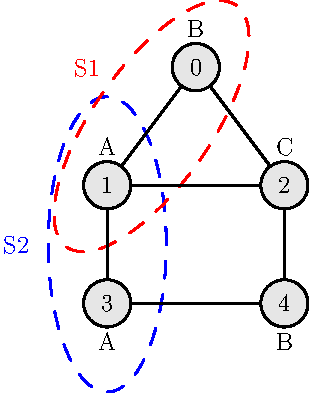
\includegraphics[width=6cm,height=7.7cm]{figure/figure-2-1}
			\caption{Labeled graph with $|V| = 5$ and $|E| = 6$}
		\end{minipage}\hfill
	\end{figure}

	We want to calculate the similarity between the two set $S_{1} = \{0,1\}$ and $S_{2} = \{1, 3\}$ using their $3$-grams:
	
	\begin{equation*}
		L(S_{1}) = [aab, acb, baa, bca, bca, bcb, cab, cba]
	\end{equation*}
	\begin{equation*}
		L(S_{2}) = [baa, baa, bca, bca, caa, cba, cba]
	\end{equation*}
	
	% Their union and intersection:
	
	% \begin{equation*}
	% L(S_{1}) \cup L(S_{2}) = [aab, acb, baa, bca, bca, bcb, cab, cba]
	% \end{equation*}
	% \begin{equation*}
	% L(S_{1}) \cap L(S_{2}) = [baa, baa, bca, bca, caa, cba, cba]
	% \end{equation*}
	
	
	So we have that:
	
	\begin{equation*}
		FJ(S_{1}, S_{2}) = \frac{4}{11}
	\end{equation*}
	
	\begin{equation*}
		BC(S_{1}, S_{2}) = \frac{8}{15}
	\end{equation*}
	
\end{esempio}

\clearpage

%%%%%%%%%%%%%%%%%%%%%%%%%%%%%%%%%%%%%%%%%%%%%%%%%%%%%%%%%%%%%%%%%%%%%%%%
%%%%%%%%%%%%%%%%%%%%%%%%%%%%%%%%%%%%%%%%%%%%%%%%%%%%%%%%%%%%%%%%%%%%%%%%
\section{Sketches}

\clearpage

%%%%%%%%%%%%%%%%%%%%%%%%%%%%%%%%%%%%%%%%%%%%%%%%%%%%%%%%%%%%%%%%%%%%%%%%
%%%%%%%%%%%%%%%%%%%%%%%%%%%%%%%%%%%%%%%%%%%%%%%%%%%%%%%%%%%%%%%%%%%%%%%%
\subsection*{Min-wise permutation}

\clearpage

%%%%%%%%%%%%%%%%%%%%%%%%%%%%%%%%%%%%%%%%%%%%%%%%%%%%%%%%%%%%%%%%%%%%%%%%
%%%%%%%%%%%%%%%%%%%%%%%%%%%%%%%%%%%%%%%%%%%%%%%%%%%%%%%%%%%%%%%%%%%%%%%%
\subsection*{Bottom-k sketches}

\clearpage

%%%%%%%%%%%%%%%%%%%%%%%%%%%%%%%%%%%%%%%%%%%%%%%%%%%%%%%%%%%%%%%%%%%%%%%%
%%%%%%%%%%%%%%%%%%%%%%%%%%%%%%%%%%%%%%%%%%%%%%%%%%%%%%%%%%%%%%%%%%%%%%%%
\section{Color Coding}

\cite{Alon:1995:COL:210332.210337}

\clearpage
